\chapter{Diseño}
\label{chapter:diseno}


El diseño de software consiste en resolver un problema planificando una eficaz solución de software. Luego de establecer el propósito y las especificaciones de los requerimientos del sistema, los desarrolladores emplearán el diseño para desarrollar la mejor solución posible que permita resolver el problema eficientemente. 

En cualquier proceso de diseño existen dos fases importantes: la diversificación y la convergencia. La diversificación es la adquisición de un repertorio de alternativas, de un material primitivo de diseño: componentes, soluciones de componentes y conocimiento, todo dentro de catálogos, de libros de texto y en la mente. Durante la convergencia, el diseñador elige y combina los elementos adecuados y extraídos de este repertorio para satisfacer los objetivos del diseño, de la misma manera a como se establece en el documento de los requisitos, y de la manera en que se acordó con el cliente. La segunda fase es la eliminación gradual de cualquier configuración de componentes excepto de una en particular, y de aquí la creación del producto final.

En términos generales, lo que pretende el diseño es brindar una visión arquitectónica o estructural de la solución planteada mostrando las interrelaciones de los componentes de mayor nivel, conocido como diseño de alto nivel, y a su vez especificar en detalles los componentes de implementación y operaciones lógicas implicadas en los niveles inferiores, conocido como diseño de bajo nivel.

Desde el comienzo de esta etapa se tuvieron en cuenta los cinco principios básicos de la programación orientada a objetos, comúnmente conocido como SOLID (Single responsibility, Open-closed, Liskov substitution, Interface segregation and Dependency inversion), los cuales, siempre y cuando se respeten, permiten construir software sencillo de mantener y que puede ser extendido fácilmente.

A continuación se resumen los cinco principios mencionados:
\begin{itemize}
\item \textbf{Single Responsibility Principle (SRP)}: cada elemento, ya sean paquetes, clases, métodos e incluso bloques de código, debería tener una única razón para cambiar. Esto significa que debe tener una única responsabilidad: ocuparse de una única tarea para aumentar de esa forma la cohesión y reducir el acoplamiento.
\item \textbf{Open/Closed Principle (OCP)}: una clase debe permitir ser extendida sin necesitar ser modificada. Es decir, que todo componente debe estar abierto a nuevas funcionalidades, pero cerrado a cambios en su código. 
\item \textbf{Liskov Substitution Principle (LSP)}: los objetos de una clase deberían poder sustituirse por instancias de las clases derivadas. 
\item \textbf{Interface Segregation Principle (ISP)}: crear pequeñas interfaces específicas para los clientes. Otra forma de expresarlo es que las clases que implementen una interfaz o una clase abstracta no deberían estar obligadas a implementar métodos que no utilizan.
\item \textbf{Dependency Inversion Principle (DIP)}: las abstracciones no deben depender de los detalles, los detalles deben depender de las abstracciones.
\end{itemize}


\section{Diseño de alto nivel}

Desde el punto de vista de la ingeniería de software, el diseño de alto nivel es una etapa crucial del desarrollo de software. Sus implicaciones y deficiencias afectan directamente al proyecto a lo largo de su ciclo de vida, por lo que la toma de decisiones en esta etapa es una tarea que debe ser llevada a cabo con mucha cautela.

\subsection{Capa de distribución (L1)}

Considerando que FuD-BOINC implementa una nueva capa de distribución del framework FuD, y que éste ya cuenta con un diseño definido al igual que BOINC, para este proyecto no se tuvo que realizar un diseño de alto nivel sino que se debió adaptar a los diseños provistos por ambos frameworks. Para ello, fue muy importante enfocarse ampliamente en la captura de requerimientos para conocer en detalle las características de los frameworks involucrados, para que al llegar a esta etapa se lograra construir una solución simple y eficaz en lo que respecta a esta adaptación.

La idea principal aquí fue de ajustar esta solución de manera que no afecte el diseño heredado de FuD manteniendo así la compatibilidad con aplicaciones que actualmente utilizan la librería. 

A continuación, las figuras \ref{fig:server-L1} y \ref{fig:cliente-L1} muestran el diseño de la capa L1 de FuD en donde se incluyen las clases con las cuales se trabajó en este proyecto:

\begin{landscape}
	\begin{figure}[H]
		\begin{center}
  			\vspace{100pt}
  			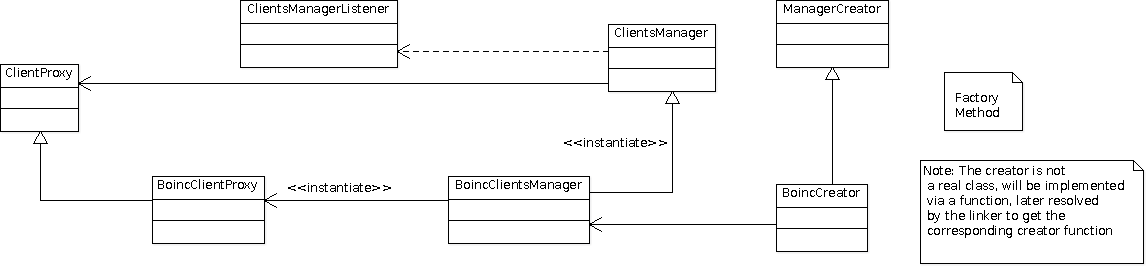
\includegraphics[scale=0.45]{images/Server_FuD-BOINC.png}
			\caption{Diseño de la capa de distribución del lado servidor}
			\label{fig:server-L1}
			\end{center}
	\end{figure} 

	\begin{figure}[H]
		\begin{center}
  			\vspace{100pt}
  			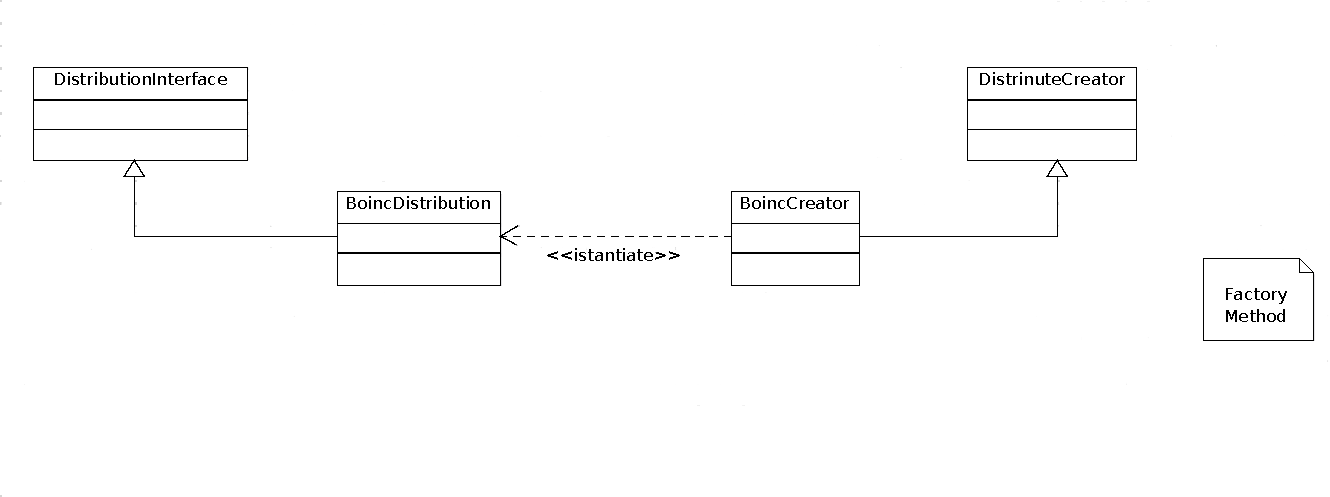
\includegraphics[scale=0.45]{images/Client_FuD-BOINC.png}
			\caption{Diseño de la capa de distribución del lado cliente}
			\label{fig:cliente-L1}
			\end{center}
	\end{figure} 
\end{landscape}

\subsection{Interacción entre FuD y BOINC}

Como se mencionó anteriormente, se hizo un trabajo de investigación muy importante que nos permitió determinar el tipo de interacción que debería existir entre FuD y BOINC. Por eso, fue necesario diferenciar correctamente la funcionalidad de cada uno de los módulos de ambos frameworks, y cómo ellos debían relacionarse.

En una primera instancia, se hizo un análisis abstracto que permitió dar un panorama general sobre cómo debían interactuar ambos frameworks. La figura \ref{fig:interaccion-fud-boinc-general} muestra dicha interacción en donde puede observarse que la capa inferior L1 de FuD-server es la encargada de comunicarse con el servidor BOINC el cual, a su vez, mantiene una comunicación con cada cliente por medio de BOINC Manager quien es el encargado de ejecutar la aplicación cliente de FuD pasándole el mensaje recibido. Lo mismo ocurre en el camino inverso desde el cliente al servidor, donde éste último recibe los resultados de la computación por parte del cliente. 

\begin{figure}[H]
	\begin{center}
  		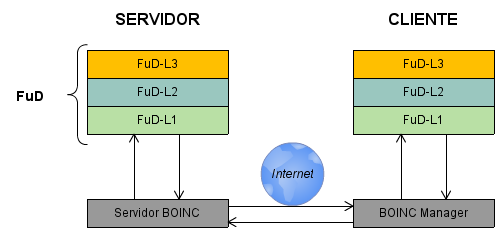
\includegraphics[scale=0.7]{images/interaccion-fud-boinc-general.png}
		\caption{Esquema general de comunicación entre FuD y BOINC}
		\label{fig:interaccion-fud-boinc-general}
	\end{center}
\end{figure}

El siguiente paso fue realizar un diagrama de secuencia que detallara aún más la interacción entre los módulos de FuD y BOINC necesarios para el cálculo de una \texttt{JobUnit}. La interacción exhibida en la figura \ref{fig:interaccion-fud-boinc} se repite por cada \texttt{JobUnit} que necesite ser computada.

\begin{landscape}
	\begin{figure}[H]
		\begin{center}
	  		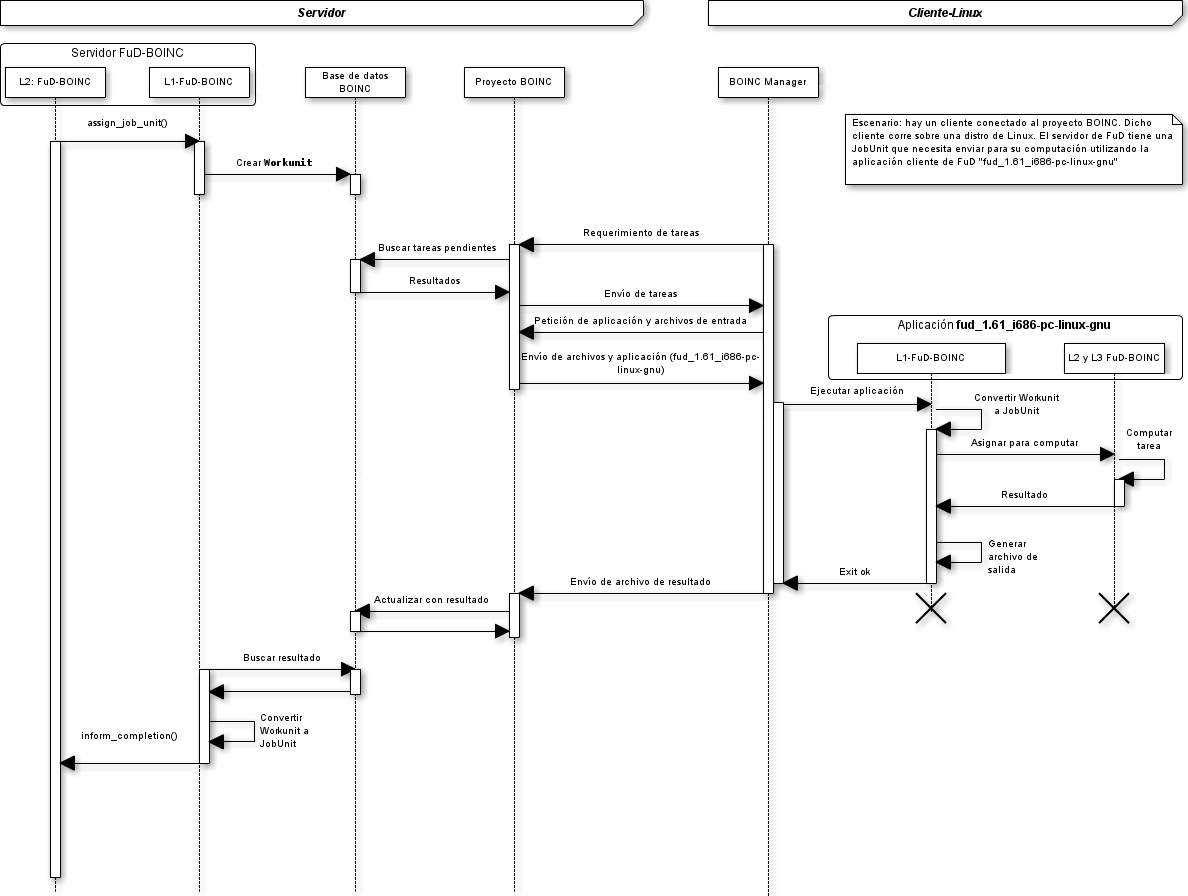
\includegraphics[scale=0.41]{images/interaccion-fud-boinc.png}
			\caption{Interacción necesaria entre FuD y la arquitectura BOINC para el cómputo de una \texttt{JobUnit}}
			\label{fig:interaccion-fud-boinc}
		\end{center}
	\end{figure}
\end{landscape}


\section{Diseño de bajo nivel}

Aquí se hace un refinamiento de las decisiones de diseño sobre aquellos componentes abstractos presentes en el diseño de alto nivel. También se analiza cómo estas clases están compuestas: los atributos de cada una, los métodos que declara y su interacción con el resto del sistema.

Para el desarrollo de FuD-BOINC, el mayor esfuerzo se debió enfocar en esta parte del diseño debido a que a partir de la vista estructural de la capa de distribución de FuD se tuvieron que especificar los nuevos módulos como así también sus principales variables y funciones. 

A continuación se muestran las clases que componen el diseño de FuD-BOINC:

\subsection{Servidor}

\subsubsection{BoincClientsManager}
\label{section:BoincClientsManager}
Es una clase que hereda directamente de la clase \texttt{ClientsManager} de FuD y está encargada del manejo de clientes del mismo. Si bien esta caractersística de múltiples clientes se hereda de FuD, la realidad es que FuD-BOINC solo debe administrar un único cliente conectado y disponible permanentemente. La existencia de un único cliente conectado permite que L2 asigne las \texttt{JobUnits} inmediatamente a L1 la cual las deberá reflejar acordemente en la base de datos del proyecto BOINC. Luego, es el framework de BOINC el encargado de realizar las conexiones con los clientes finales (voluntarios) para el envío dichas tareas.

Además, como el servidor del proyecto BOINC se encarga de reenviar aquellas tareas fallidas o no computadas, para esta implementación fue necesario deshabilitar el reenvío de \texttt{JobUnits} por parte de FuD ya que por defecto son reenviadas cuando las mismas no son informadas. 
Por lo tanto, al heredar de \texttt{ClientsManager} se debió proveer de esta funcionalidad, que en este caso fue introducida al realizar el rediseño de FuD descripto en la sección \ref{seccion:rediseno:fud}:

\begin{itemize}
\item \texttt{bool should\_resend\_job\_units()}: su función es determinar si la implementación de la capa L1 permite el reenvío de \texttt{JobUnits}. Este método es utilizado por el \texttt{JobManager}, perteneciente a la capa L2 de FuD, para determinar si debe volver a enviar aquellas \texttt{JobUnits} que aún no fueron reportadas por los nodos de procesamiento.
\end{itemize}

La figura \ref{fig:BoincClientsManager} muestra el diseño de la clase \texttt{BoincClientsManager}:

\begin{figure}[H]
	\begin{center}
  		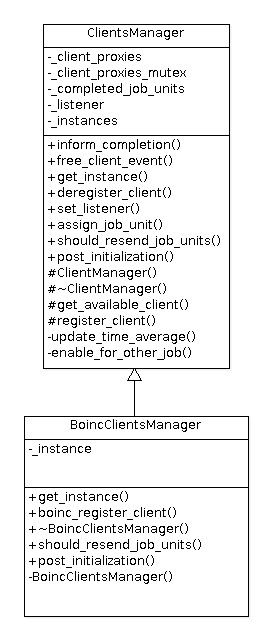
\includegraphics[scale=0.65]{images/BoincClientsManager.png}
		\caption{Clase BoincClientsManager}
		\label{fig:BoincClientsManager}
		\end{center}
\end{figure} 


\subsubsection{BoincClientProxy}

La clase \texttt{BoincClientProxy} hereda directamente de la clase \texttt{ClientProxy} de FuD y representa a un cliente conectado para la capa L1 de éste framework; en el caso de esta implementación, una instancia de \texttt{BoincClientProxy} representa una conexión con el servidor de BOINC, más precisamente con su base de datos.

Su función principal es la de crear y mantener una conexión directa con el servidor BOINC por medio de la cual notificará sobre las tareas a computar y se encargará de obtener los resultados recibidos de las computaciones realizadas por los voluntarios del proyecto. 

Como se dijo en el punto anterior, para representar la existencia de un único cliente conectado es importante que exista una única instancia de esta clase que será manejada por \texttt{BoincClientsManager}.

Es importante dejar en claro que el hecho de que FuD-BOINC considere disponible en todo momento al servidor de BOINC no implica que dicho servidor esté corriendo o detenido ya que la comunicación de la capa L1 se realiza directamente con la base de datos del proyecto. De esta manera, el servidor de FuD-BOINC podría correr y generar tareas en la base de datos del proyecto las cuales serán enviadas a los clientes una vez que el servidor sea iniciado.

La estructura de \texttt{BoincClientProxy} puede verse en la figura \ref{fig:BoincClientProxy}:

La funcionalidad heredada que debe ser provista a FuD mediante esta clase es la siguiente:

\begin{itemize}
\item \texttt{void process(const JobUnit\& job\_unit)}: su función es enviar la \texttt{JobUnit} a un cliente para su procesamiento. La implementación de este método depende del tipo de \texttt{ClientsManager} utilizado, en este caso \texttt{BoincClientsManager}.
\end{itemize}

\begin{figure}[H]
	\begin{center}
  		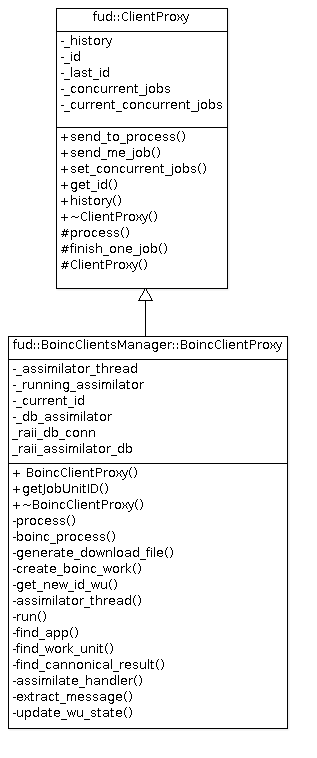
\includegraphics[scale=0.65]{images/BoincClientProxy.png}
		\caption{Clase BoincClientProxy}
		\label{fig:BoincClientProxy}
	\end{center}
\end{figure} 


\subsection{Cliente}

\subsubsection{BoincDistribution}
\label{seccion:diseno:BoincDistribution}
Esta clase hereda de la clase abstracta \texttt{DistributionClient} de FuD y provee la funcionalidad necesaria para la comunicación con el servidor. En el caso de este proyecto, la comunicación directa entre cliente y servidor de FuD no existe ya que BOINC es el encargado de llevar a cabo dicha tarea. Por el contrario, esta clase es la encargada de interpretar la \texttt{workunit} brindada por BOINC Manager \ref{boinc:manager} cuando éste ejecuta la aplicación cliente de FuD. Luego, al finalizar la computación de la tarea, se ocupa de escribir los resultados en un archivo de salida para que BOINC Manager lo informe al servidor.

Básicamente, su función es de traducir la \texttt{workunit} de BOINC a \texttt{JobUnit}, informar de la \texttt{JobUnit} a su capa superior, y luego realizar el proceso inverso.

La figura \ref{fig:BoincDistribution} muestra el diseño de esta clase:

\begin{figure}[H]
	\begin{center}
  		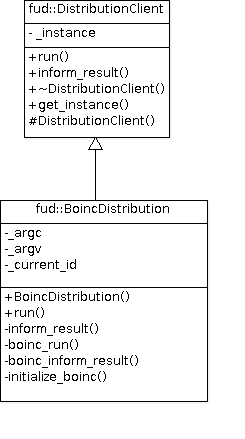
\includegraphics[scale=0.65]{images/BoincDistribution.png}
		\caption{Clase BoincDistribution}
		\label{fig:BoincDistribution}
	\end{center}
\end{figure}

Las funcionalidades más importantes de \texttt{BoincDistribution} deben ser provistas por los siguientes métodos:

\begin{itemize}
\item \texttt{void run()}: es el método encargado de iniciar la comunicación con el server. En este caso, se encarga de iniciar el proceso de traducción de la \texttt{workunit} a \texttt{JobUnit}.
\item \texttt{void inform\_result(bool result)}: su función es la de informar al servidor el resultado de la computación. En este caso, se encarga de escribir el resultado en un archivo binario.
\item \texttt{fud::create\_distribution\_client(int argc, char** argv)}: método encargado de la creación de una instancia de \texttt{DistributionClient}. En este caso, se crea una instancia de \texttt{BoincDistribution}.
\end{itemize}
